\usetikzlibrary{calc,angles}
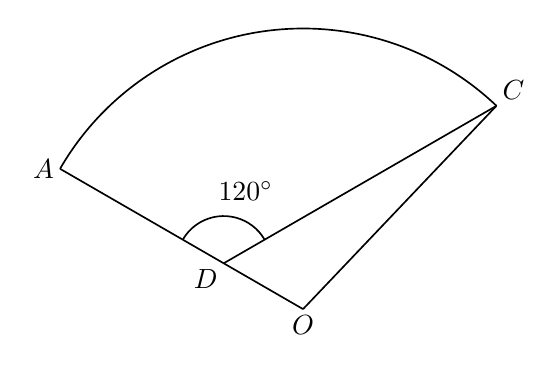
\begin{tikzpicture}[x=.8cm,y=.8cm,font=\normalsize,
  geometry edge/.style={solid,line width=.6pt},
  geometry label/.style={font=\normalsize,inner sep=2pt}]
  \coordinate (D) at (0,0);
  \coordinate (A) at (-2.598076211353,1.5);
  \coordinate (O) at (1.259673314596,-0.727272727273);
  \coordinate (C) at (4.330127018922,2.5);
  \draw[geometry edge] (O)--(A);
  \draw[geometry edge] (D)--(C);
  \draw[geometry edge] (O)--(C);
  \draw[geometry edge] (A) arc[start angle=150,end angle=46.426421,radius=4.454545455];
  \draw[geometry edge] (D) ++(30:0.75) arc[start angle=30,end angle=150,radius=0.75];
  \node[geometry label] at (0.35,1.15) {$120^\circ$};
  \node[geometry label,left] at (A) {$A$};
  \node[geometry label,above right] at (C) {$C$};
  \node[geometry label,below left] at (D) {$D$};
  \node[geometry label,below] at (O) {$O$};
\end{tikzpicture}
